


\begin{SCfigure*}
	\centering
	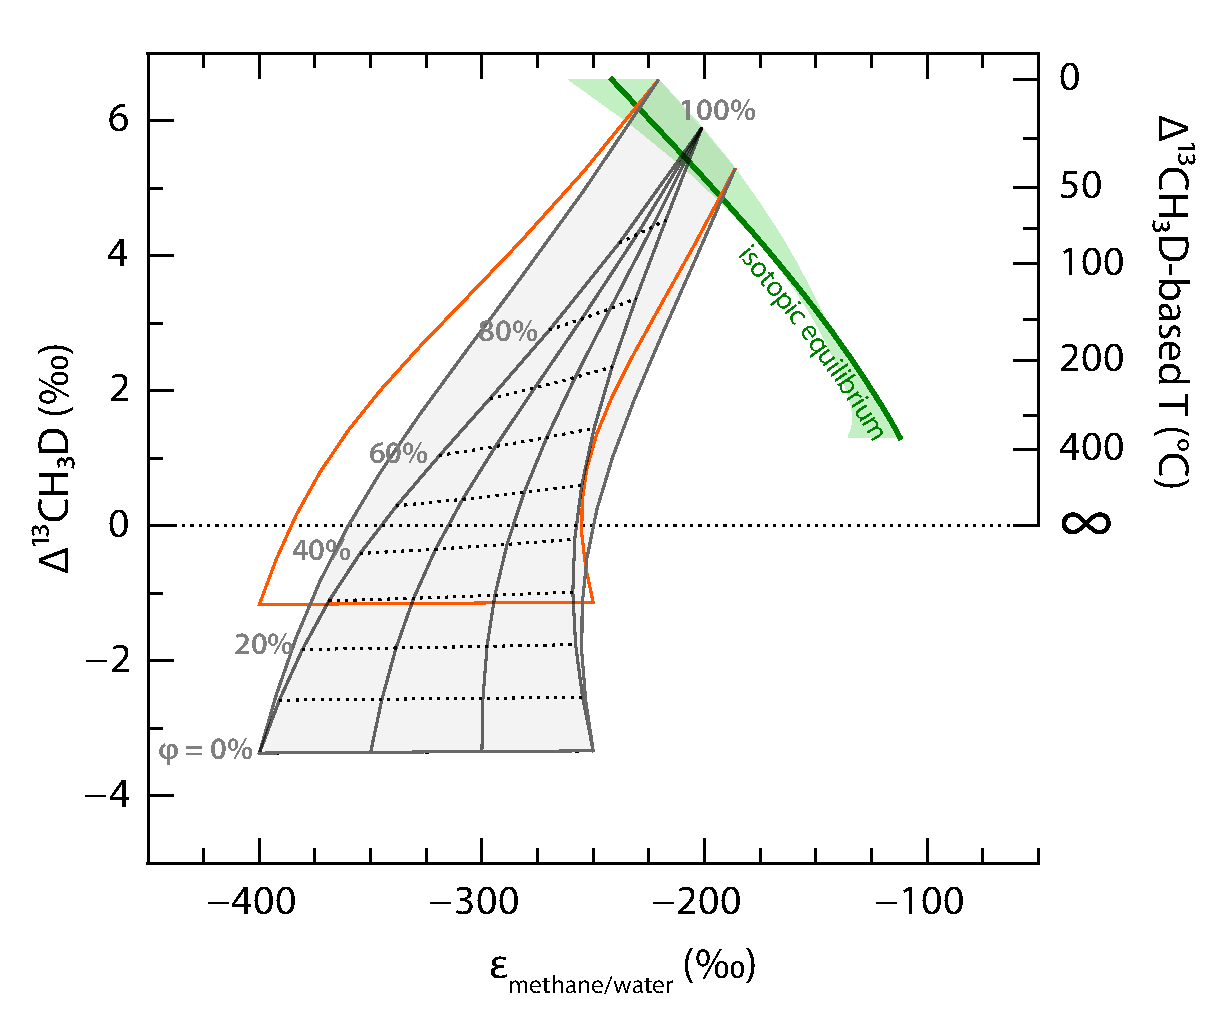
\includegraphics[width=0.5\linewidth]{figures/Fig2.S5}
	\caption[Dependence of model predictions on reversibility and fractionation
	factors]{Dependence of the modeled isotopic composition of microbial
		methane on the degree of reversibility and isotope fractionation
		factors. Orange and gray fields represent model output assuming a
		kinetic endmembers of $-$1.3‰ and $-$3.5‰, respectively (\autoref{tab:2:S3}). Inner
		solid gray lines represent model trajectories for 20~°C assuming
		different values for the D/H primary intrinsic isotope effect (\autoref{tab:2:S3}). Subhorizontal tie lines connect points of equal reversibility ($\varphi$).
		Outer solid lines represent bounding model trajectories calculated for 0
		and 40~°C.}
	\label{fig:2:S5}
\end{SCfigure*}